\begin{exercice*}
    Comparer chaque figure à la figure grise et remplir le tableau.
    
    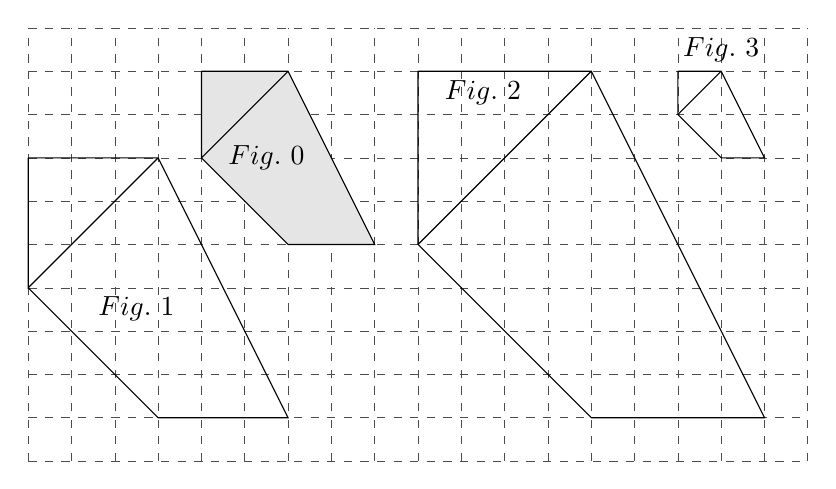
\begin{tikzpicture}[scale = 0.55]
            \draw[help lines, color=black!70, dashed] (0,0) grid (18,10);                            
            % Fig0
            \coordinate (A0) at (4,9);
            \coordinate (B0) at (6,9);
            \coordinate (C0) at (8,5);
            \coordinate (D0) at (6,5);
            \coordinate (E0) at (4,7);            
            \fill[color=black!10] (A0)--(B0)--(C0)--(D0)--(E0)--(A0);
            \draw (A0)--(B0)--(C0)--(D0)--(E0)--(A0)--(E0)--(B0);
            \coordinate[label=above:$Fig.~0$] (F0) at (5.5,6.5);        
            % Fig1
            \coordinate[label=above:$Fig.~1$] (F1) at (2.5,3);                    
            \coordinate (A) at (0,7);
            \coordinate (B) at (3,7);
            \coordinate (C) at (6,1);
            \coordinate (D) at (3,1);
            \coordinate (E) at (0,4);
            \draw (A)--(B)--(C)--(D)--(E)--(A)--(E)--(B);
            % Fig2
            \coordinate[label=above:$Fig.~2$] (F2) at (10.5,8);        
            \coordinate (A2) at (9,9);
            \coordinate (B2) at (13,9);
            \coordinate (C2) at (17,1);
            \coordinate (D2) at (13,1);
            \coordinate (E2) at (9,5);
            \draw (E2)--(B2);
            \draw (A2)--(B2)--(C2)--(D2)--(E2)--(A2);        
            % Fig3
            \coordinate[label=above:$Fig.~3$] (F3) at (16,9);        
            \coordinate (A3) at (15,9);
            \coordinate (B3) at (16,9);
            \coordinate (C3) at (17,7);
            \coordinate (D3) at (16,7);
            \coordinate (E3) at (15,8);
            \draw (E3)--(B3);
            \draw (A3)--(B3)--(C3)--(D3)--(E3)--(A3);                
    \end{tikzpicture}

    \begin{tabular}{|c|>{\centering\arraybackslash}m{0.4\linewidth}|*{2}{>{\centering\arraybackslash}m{0.25\linewidth}|}}        
        \cline{2-4}
        \multicolumn{1}{c|}{}
        &Agrandissement&Réduction&Rapport\\\hline
        Fig.1&&&\\\hline
        Fig.2&&&\\\hline
        Fig.3&&&\\\hline
    \end{tabular}    
\end{exercice*}
\begin{corrige}
%\setcounter{partie}{0} % Pour s'assurer que le compteur de \partie est à zéro dans les corrigés
% \phantom{rrr}  
    Comparer chaque figure à la figure grise et remplir le tableau.

    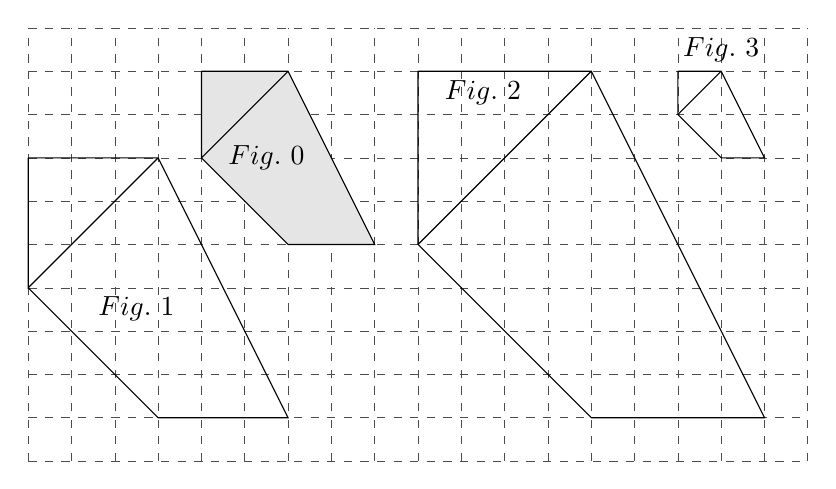
\begin{tikzpicture}[scale = 0.55]
            \draw[help lines, color=black!70, dashed] (0,0) grid (18,10);                            
            % Fig0
            \coordinate (A0) at (4,9);
            \coordinate (B0) at (6,9);
            \coordinate (C0) at (8,5);
            \coordinate (D0) at (6,5);
            \coordinate (E0) at (4,7);            
            \fill[color=black!10] (A0)--(B0)--(C0)--(D0)--(E0)--(A0);
            \draw (A0)--(B0)--(C0)--(D0)--(E0)--(A0)--(E0)--(B0);
            \coordinate[label=above:$Fig.~0$] (F0) at (5.5,6.5);        
            % Fig1
            \coordinate[label=above:$Fig.~1$] (F1) at (2.5,3);                    
            \coordinate (A) at (0,7);
            \coordinate (B) at (3,7);
            \coordinate (C) at (6,1);
            \coordinate (D) at (3,1);
            \coordinate (E) at (0,4);
            \draw (A)--(B)--(C)--(D)--(E)--(A)--(E)--(B);
            % Fig2
            \coordinate[label=above:$Fig.~2$] (F2) at (10.5,8);        
            \coordinate (A2) at (9,9);
            \coordinate (B2) at (13,9);
            \coordinate (C2) at (17,1);
            \coordinate (D2) at (13,1);
            \coordinate (E2) at (9,5);
            \draw (E2)--(B2);
            \draw (A2)--(B2)--(C2)--(D2)--(E2)--(A2);        
            % Fig3
            \coordinate[label=above:$Fig.~3$] (F3) at (16,9);        
            \coordinate (A3) at (15,9);
            \coordinate (B3) at (16,9);
            \coordinate (C3) at (17,7);
            \coordinate (D3) at (16,7);
            \coordinate (E3) at (15,8);
            \draw (E3)--(B3);
            \draw (A3)--(B3)--(C3)--(D3)--(E3)--(A3);                
    \end{tikzpicture}
    
    \smallskip
    
    \begin{tabular}{|c|*{3}{>{\centering\arraybackslash}m{0.25\linewidth}|}}        
        \cline{2-4}
        \multicolumn{1}{c|}{}
        &Agrandissement&Réduction&Rapport\\\hline
        {\color{black}Fig.1}&{\color{red} oui}&{\color{red} non}&{\color{red} \num{1.5}}\\\hline
        Fig.2&{\color{red} oui}&{\color{red} non}&{\color{red} \num{2}}\\\hline
        Fig.3&{\color{red} non}&{\color{red} oui}&{\color{red} \num{0.5}}\\\hline
    \end{tabular}
\end{corrige}

